\begin{pastexam}[label={px:ntu-106-ie-ds-11}]{臺大工工所 106 學年度 第 11 題}
（複選；每題 10 分，每個選項單獨計分，答對 2 分，答錯倒扣 2 分）

Given an AVL tree as shown below, let T$_1$, T$_2$, T$_3$ and T$_4$ be full binary sub-trees with
heights equal to $h$, $h$-1, $h$-1, and $h$, respectively. If we insert a series of nodes orderly to the
leaves of T$_4$, T$_3$, T$_2$, and T$_1$, one node to each sub-tree at a time, then after rotation(s) and
re-balancing, which of the following is(are) true?

\begin{center}
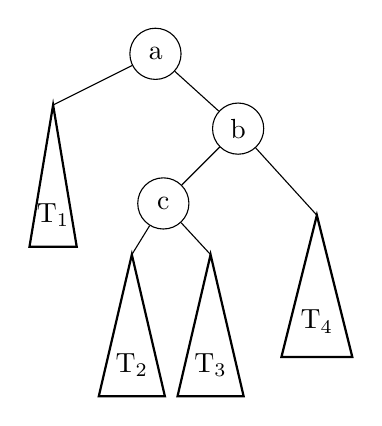
\begin{tikzpicture}[v/.style={circle,draw,inner sep=1pt,minimum size=6.5mm},
  tri/.style={draw,thick,line join=miter}]
\node[v] (a) at (0,0) {a};
\node[v] (b) at (1.05,-0.95) {b};
\node[v] (c) at (0.1,-1.9) {c};
\draw[tri] (-1.3,-0.65) -- (-1.6,-2.45) -- (-1.0,-2.45) -- cycle;
\node at (-1.3,-2.05) {T$_1$};
\draw[tri] (-0.3,-2.55) -- (-0.72,-4.35) -- (0.12,-4.35) -- cycle;
\node at (-0.3,-3.95) {T$_2$};
\draw[tri] (0.7,-2.55) -- (0.28,-4.35) -- (1.12,-4.35) -- cycle;
\node at (0.7,-3.95) {T$_3$};
\draw[tri] (2.05,-2.05) -- (1.6,-3.85) -- (2.5,-3.85) -- cycle;
\node at (2.05,-3.4) {T$_4$};
\draw (a) -- (-1.3,-0.65);
\draw (a) -- (b);
\draw (b) -- (c);
\draw (b) -- (2.05,-2.05);
\draw (c) -- (-0.3,-2.55);
\draw (c) -- (0.7,-2.55);
\end{tikzpicture}
\end{center}
\begin{enumerate}[label=(\Alph*),nosep]
\item There are totally two single rotations encountered during these insertions.
\item Node `c' will be the root of the resultant AVL tree.
\item `b' will be the parent of `a'.
\item The roots of the sub-trees T$_2$ and T$_3$ are sibling nodes of a common parent.
\item If we insert another node to the leaf of T4, the AVL tree will become unbalanced again.
\end{enumerate}
\end{pastexam}

\begin{pastsoln}
答案：(C)(D)。

\textbf{解讀}。 「insert a series of nodes orderly to the leaves of T$_4$, T$_3$, T$_2$, and T$_1$, one node to each
sub-tree at a time」讀成：依序插入四個節點，第一個落在 T$_4$ 的某個葉子底下，第二個落在 T$_3$，第三個 T$_2$，
第四個 T$_1$。 高度照資結書第~7.1~節的約定數層數；T$_i$ 是完美（full）二元樹，在它的葉子底下多接一個節點，
它的高度就加 1，而子樹內部仍然平衡（每個節點左右只差 0 或 1）。 為了讓 T$_2$、T$_3$ 不是空樹，設 $h \ge 2$。

\textbf{原來的高度}：c 的左右是 $h-1$、$h-1$，c 高 $h$；b 的左右是 c（$h$）、T$_4$（$h$），b 高 $h+1$；
a 的左右是 T$_1$（$h$）、b（$h+1$），a 高 $h+2$，右邊高 1，平衡。

\textbf{第 1 個插入 T$_4$}：T$_4$ 變 $h+1$。 b 的左右 $h$、$h+1$，b 變 $h+2$；a 的左右 $h$、$h+2$，
差 2，a 失衡。 新節點在 a 的右子節點 b 的右子樹裡，是 RR 型，在 a 做一次左旋（單旋轉，資結書第~10.2.3~節）：
b 上來當根，a 變成 b 的左子節點，b 原來的左子樹 c 改接成 a 的右子樹。
\begin{center}
\begin{tikzpicture}[v/.style={circle,draw,inner sep=1pt,minimum size=6.5mm},
  t/.style={draw,isosceles triangle,shape border rotate=90,inner sep=1pt,minimum height=8mm,font=\small},
  level distance=11mm, level 1/.style={sibling distance=34mm}, level 2/.style={sibling distance=18mm},
  level 3/.style={sibling distance=10mm}]
\node[v] {b}
  child {node[v] {a}
    child {node[t] {T$_1$}}
    child {node[v] {c} child {node[t] {T$_2$}} child {node[t] {T$_3$}}}}
  child {node[t] {T$_4$}};
\end{tikzpicture}
\end{center}
旋轉後：c 高 $h$；a 的左右 T$_1$（$h$）、c（$h$），a 高 $h+1$；b 的左右 a（$h+1$）、T$_4$（$h+1$），b 高 $h+2$，平衡。

\textbf{第 2 個插入 T$_3$}：T$_3$ 變 $h$。 c 的左右 $h-1$、$h$，c 變 $h+1$；a 的左右 $h$、$h+1$，a 變 $h+2$；
b 的左右 $h+2$、$h+1$，b 變 $h+3$。 每個節點左右只差 1，不用旋轉。

\textbf{第 3 個插入 T$_2$}：T$_2$ 變 $h$。 c 的左右 $h$、$h$，c 的高度仍是 $h+1$，往上的高度都不變，不用旋轉。

\textbf{第 4 個插入 T$_1$}：T$_1$ 變 $h+1$。 a 的左右 $h+1$、$h+1$，a 的高度仍是 $h+2$，不用旋轉。

最後的樹就是上圖的形狀：b 是根，a 是 b 的左子節點，a 的左右是 T$_1$、c，c 的左右是 T$_2$、T$_3$，b 的右邊是 T$_4$。
整個過程只有第 1 次插入做了一次單旋轉。

\textbf{逐項}：
\begin{itemize}
\item (A) 錯。 只有一次單旋轉，不是兩次。
\item (B) 錯。 根是 b，c 在第三層。
\item (C) 對。 旋轉後 a 是 b 的左子節點，之後沒有再改變。
\item (D) 對。 T$_2$、T$_3$ 的根都是 c 的子節點，是兄弟。
\item (E) 錯。 現在 b 的左邊高 $h+2$、右邊 T$_4$ 高 $h+1$。 再插一個到 T$_4$，T$_4$ 最多變成 $h+2$，b 的左右相等，
a、b 都不會失衡。 T$_4$ 內部會不會失衡要看插在哪個葉子：接在第 1 次新加的那個節點底下，T$_4$ 裡面那個節點會差 2，
要在 T$_4$ 裡旋轉一次；接在 T$_4$ 其他原來的葉子底下，則完全不會失衡。 「will become unbalanced」說一定會，不成立。
\end{itemize}
\end{pastsoln}
